\newpage
\section{Hotspot Analysis}
The goal of this analysis is to identify the parts of the program that consume the most execution time. To reach this objective, I have considered data size resulting in sequential time $\sim 30$ seconds, setting $N = 100'000$.

\subsection{Code description}
\begin{lstlisting}[caption={Pseudo code in C}]
int main() {
    int N = 100000;
    double *xr, *xi, *Xr, *Xi;

    fillInput(xr, xi, N);            // initialize input signal
    zero(Xr, Xi, N);                 // clear output buffers

    DFT(+1, xr, xi, Xr, Xi, N);      // compute DFT
    DFT(-1, Xr, Xi, xr, xi, N);      // compute IDFT

    checkResults(xr, xi, Xr, Xi, N); // verify correctness

    return 0;
}

void DFT(int idft, double* xr, ..., double* Xi, int N) {
    for (int k = 0; k < N; k++)
        for (int n = 0; n < N; n++) {
            double a = 2*M_PI*n*k/N;
            Xr[k] += xr[n]*cos(a) + idft*xi[n]*sin(a);
            Xi[k] += -idft*xr[n]*sin(a) + xi[n]*cos(a);
        }

    if (idft == -1)
        for (int n = 0; n < N; n++) {
            Xr[n] /= N;
            Xi[n] /= N;
        }
}
\end{lstlisting}

\noindent
The code implements the Discrete Fourier Transform (DFT) and its Inverse (IDFT) in C. It calculates the transform of a signal and verify the correctness through IDFT following the definition:

\[
X[k] = \sum_{n=0}^{N-1} x[n] \, e^{-j 2 \pi k n / N}, \quad k = 0,1,\dots,N-1
\]

\subsection{Sequential and Parallel Sections}
In order to apply Amdahl's Law described in the previous section, we must identify the sequential and parallel parts of the code. 
I have empirically measured these sections by running the code 10 times, separating the serial and parallel portions.
More details can be found in the code \texttt{identify\_seq\_par\_code.c}.\\

\noindent
The results are the following:

% TODO aggiungere i valori
\begin{table}[h!]
\centering
\begin{tabular}{l c}
\hline
\textbf{Quantity} & \textbf{Value} \\
\hline
Total execution time $T_\text{tot}$ & $\text{measured}$ s \\
Time of the parallelizable section $T_\text{par}$ & $\text{measured}$ s \\
Time of the serial section $T_\text{ser} = T_\text{tot} - T_\text{par}$ & $\text{computed}$ s \\
Fraction of serial code $f_s = \frac{T_\text{ser}}{T_\text{tot}}$ & $\text{computed}$ \\
\hline
\end{tabular}
\label{tab:seq_par_times}
\end{table}

\noindent
These values will be used to estimate the theoretical speedup according to Amdahl's Law:

\[
S(p) = \frac{1}{f_s + \frac{1-f_s}{p}}
\]


where $p$ is the number of threads.
% TODO aggiungere una tabella/grafico di S(p)
\begin{figure}[H]
    \centering
    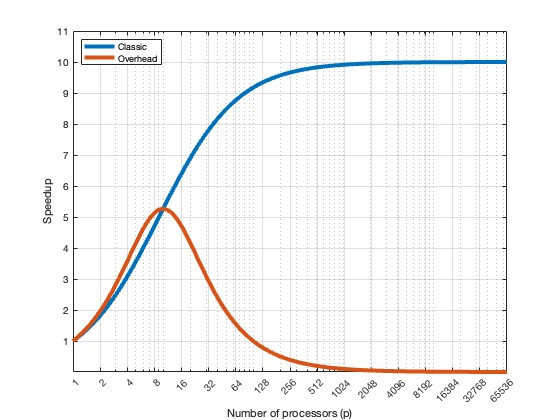
\includegraphics[width=0.7\textwidth]{assets/amdalhs_law/classic_vs_overhead.jpg}
    \label{fig:classic_vs_overhead}
\end{figure}

\paragraph{Note:} the smaller the serial fraction $f_s$, the higher the potential speedup achievable by parallelizing the main loop of the DFT.

\subsection{Hotspot Identification}
The measurements were performed using two methods: 

\begin{itemize}
    \item \textbf{Manually}: using \texttt{omp\_get\_wtime()} 
    \item \textbf{Profiler}: using \texttt{Intel VTune}
\end{itemize}

% TODO: aggiornare le tabelle
\begin{center}
    \begin{minipage}{0.48\textwidth}
    \centering
    \captionof{table}{Manually}
    \resizebox{\textwidth}{!}{%
    \begin{tabular}{lrr}
        \toprule
        Function & Time (s) & Percentage (\%) \\
        \midrule
        \csvreader[late after line=\\]{assets/hotspots/hotspots_40000_manually.csv}{}
        {\csvcoli & \csvcolii & \csvcoliii} 
        \bottomrule
    \end{tabular}%
    }
    \end{minipage}%
    \hfill
    \begin{minipage}{0.48\textwidth}
    \centering
    \captionof{table}{Intel VTune Profiler}
    \resizebox{\textwidth}{!}{%
    \begin{tabular}{lrr}
        \toprule
        Function Stack & CPU Time: Self & Percentage (\%) \\
        \midrule
        \csvreader[late after line=\\]{assets/hotspots/top-down-tree.csv}{}
        {\csvcoli & \csvcolii & \csvcoliii} 
        \bottomrule
    \end{tabular}%
    }
    \end{minipage}
\end{center}

\begin{center}
    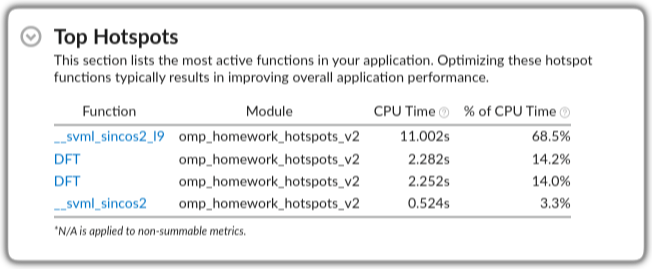
\includegraphics[width=0.8\textwidth]{assets/hotspots/top-hotspots-border.png}
\end{center}

\subsection{Conclusion}
The main hotspot is the DFT() function and its inverse IDFT(), which together account for over 99\% of the total execution time. All other functions have negligible impact. This indicates that \textbf{parallelization and vectorization efforts should focus on the double loop inside DFT()}.

\begin{figure}[ht]
    \centering
    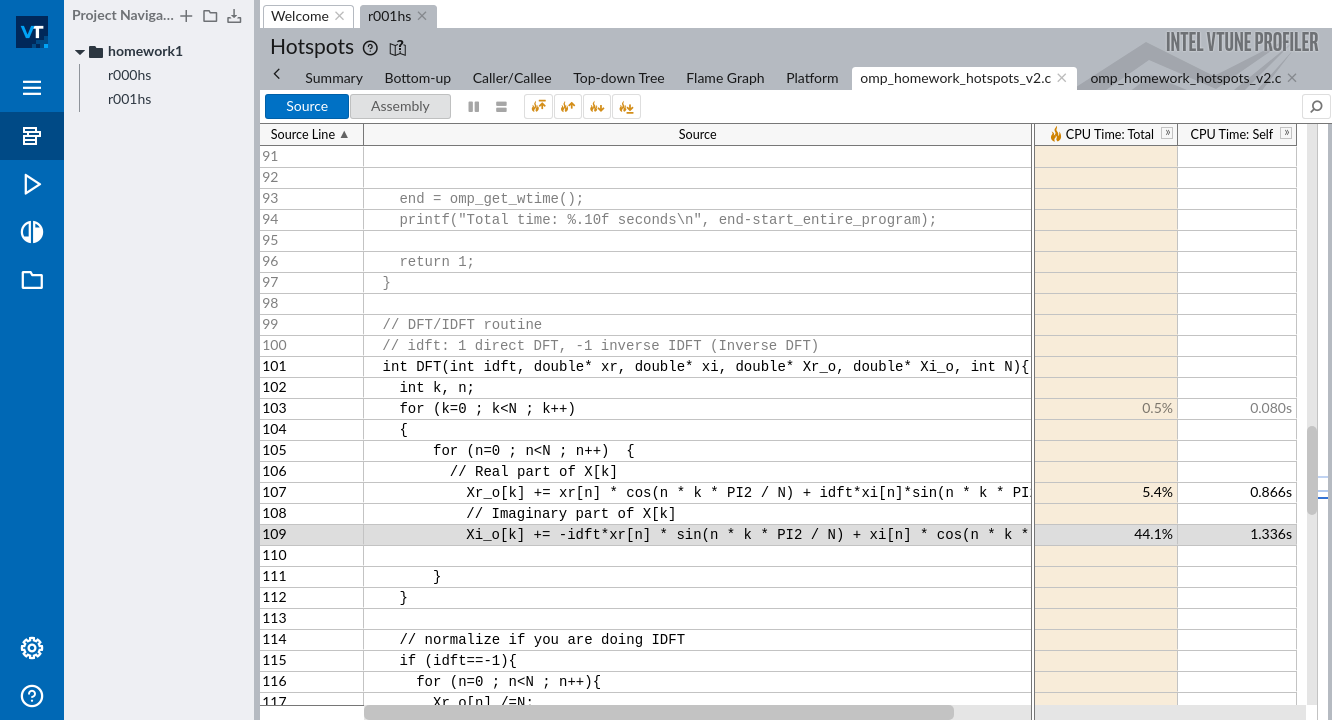
\includegraphics[width=0.9\textwidth]{assets/hotspots/vtune_biggest_hotspot_screen.png}
    \caption{The main hotspot is the loop contained in lines 103-112.}
    \label{fig:vtune_biggest_hotspot_screen}
\end{figure}
